\let\negmedspace\undefined
\let\negthickspace\undefined
\documentclass[journal]{IEEEtran}
\usepackage[a5paper, margin=10mm, onecolumn]{geometry}
%\usepackage{lmodern} % Ensure lmodern is loaded for pdflatex
\usepackage{tfrupee} % Include tfrupee package

\setlength{\headheight}{1cm} % Set the height of the header box
\setlength{\headsep}{0mm}     % Set the distance between the header box and the top of the text

\usepackage{gvv-book}
\usepackage{gvv}
\usepackage{cite}
\usepackage{amsmath,amssymb,amsfonts,amsthm}
\usepackage{algorithmic}
\usepackage{graphicx}
\usepackage{textcomp}
\usepackage{xcolor}
\usepackage{txfonts}
\usepackage{listings}
\usepackage{enumitem}
\usepackage{mathtools}
\usepackage{gensymb}
\usepackage{comment}
\usepackage[breaklinks=true]{hyperref}
\usepackage{tkz-euclide} 
\usepackage{listings}
% \usepackage{gvv}                                        
\def\inputGnumericTable{}                                 
\usepackage[latin1]{inputenc}                                
\usepackage{color}                                            
\usepackage{array}                                            
\usepackage{longtable}                                       
\usepackage{calc}                                             
\usepackage{multirow}                                         
\usepackage{hhline}                                           
\usepackage{ifthen}                                           
\usepackage{lscape}
\begin{document}

\bibliographystyle{IEEEtran}

\title{2.4.18}
\author{EE25BTECH11022 - sankeertthan}
% \maketitle
% \newpage
% \bigskip
{\let\newpage\relax\maketitle}

\renewcommand{\thefigure}{\theenumi}
\renewcommand{\thetable}{\theenumi}
\setlength{\intextsep}{10pt} % Space between text and floats


\textbf{Question}: show that the line through the points \brak{1,-1,2} , \brak{3,4,-2} is perpendicular to the line through the  points  \brak{0,3,2} and \brak{3,5,6}

\textbf{solution}:
\begin{align}
let \Vec{A} =\brak{1,-1,2},\Vec{B} =\brak{3,4,-2},\Vec{C} =\brak{0,3,2},\Vec{D} =\brak{3,5,6}
\end{align}
Direction vector of line joining points $\Vec{A}$ and $\Vec{B}$ is
\begin{align}
    \Vec{B}-\Vec{A} &= \myvec{3-1 \\ 4-(-1) \\ -2-2}\\
    &= \myvec{2 \\ 5 \\-4}\\
\end{align}
Direction vector of line joining points $\Vec{C}$ and $\Vec{D}$ is
\begin{align}
    \Vec{C}-\Vec{D} &= \myvec{3-0 \\ 5-3 \\ 6-2}\\
    &= \myvec{3 \\ 2 \\4}\\
\end{align}
\begin{align}
\myvec{\vec{B}-\vec{A}}^\top\myvec{\vec{D}-\vec{C}} &= \myvec{2 \ \ 5 \ \ -4}\myvec{3 \\ 2 \\4}\\
 &= 2\brak{3}+5\brak{2}+\brak{-4}\brak{4}\\
 &=6+10-16\\
 &=0\\
 \myvec{\vec{B}-\vec{A}}^\top\myvec{\vec{D}-\vec{C}} = 0
\end{align}
Therefore, the lines joining points $\Vec{A}$,$\Vec{B}$ and $\Vec{C}$,$\Vec{D}$ are perpendicular 

\begin{figure}
    \centering
    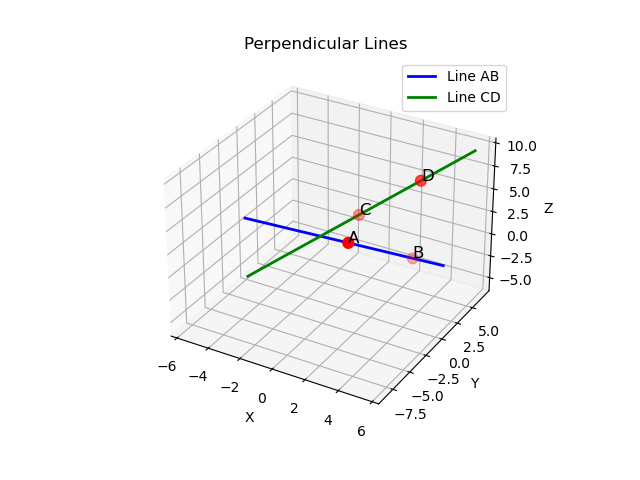
\includegraphics[width=\linewidth]{figs/points.png}
    \caption{}
\end{figure}
\end{document}